%%----------------------------------------------------------------------------
%% Onderzoekstechnieken: Het onderzoeksproces
%%----------------------------------------------------------------------------

\documentclass[aspectratio=169]{beamer}

%==============================================================================
% Aanloop
%==============================================================================

%---------- Vormgeving --------------------------------------------------------

\usetheme{hogent}

\usecolortheme{hgwhite} % witte achtergrond, zwarte tekst

\usepackage{graphicx,multicol}
\usepackage{comment,enumerate,hyperref}
\usepackage{amsmath,amsfonts,amssymb}
\usepackage[dutch]{babel}
\usepackage{multirow}
\usepackage{eurosym}
\usepackage{listings}
\usepackage{textcomp}
\usepackage{framed}
\usepackage{wrapfig}
\usepackage{tabu} %needed for \tabulinesep

%---------- Configuratie ------------------------------------------------------

\usetikzlibrary{arrows,shapes,backgrounds,positioning,shadows}

%---------- Commando-definities -----------------------------------------------

\newcommand{\tabitem}{~~\llap{\textbullet}~~}
\newcommand{\alertbox}[2][hgblue]{%
  \setbeamercolor{alertbox}{bg=#1,fg=white}
  \begin{beamercolorbox}[sep=2pt,center]{alertbox}
    \textbf{#2}
  \end{beamercolorbox}
}

%---------- Info over de presentatie ------------------------------------------

\title{Chapter 2. The Research Process}
\subtitle{Research Techniques}
\author{Jens Buysse \and Wim {De Bruyn} \and Pieter-Jan Maenhaut \and Bert {Van Vreckem}}
\date{AY 2019-2020}

%==============================================================================
% Inhoud presentatie
%==============================================================================

\begin{document}

\begin{frame}
  \maketitle
\end{frame}

\begin{frame}
  \frametitle{What's on the menu?}
  
  \tableofcontents
\end{frame}

\begin{frame}
  \frametitle{Learning Goals}
  
  \begin{itemize}
    \item The scientific method
    \item Research process
    \item Variables and measurement levels
    \item Samples
    \item Basic concepts
  \end{itemize}
\end{frame}

\section{The Scientific Method}


\begin{frame}[plain]
  \bfseries\Large
  No matter how many instances of white swans we may have observed, this does not justify the conclusion that all swans are white
  
  \bigskip
  
  ---Karl Popper
\end{frame}

\begin{frame}[plain]
  \centering
  \includegraphics[height=\textheight]{les1-01}
\end{frame}

\begin{frame}
  \frametitle{How do we gain knowledge?}
  
  \centering
  \includegraphics[height=.8\textheight]{les1-02}
\end{frame}

\begin{frame}[plain,c]
  \begin{columns}
    \column{\dimexpr\paperwidth}
    \includegraphics[width=\paperwidth]{les1-03}
  \end{columns}
\end{frame}

\begin{frame}
  \frametitle{How do we gain knowledge?}
  
  \begin{columns}[c]
    
    \column{.5\textwidth}
    Non-scientific method
    \begin{itemize}
      \item ``My gut feeling says so''
      \item ``My father says so, so it must be true''
      \item ``There are many reports of UFO sightings, so there must be alien life''
      \item ``I read it on the Internet!''
    \end{itemize}
    
    \pause
    
    \column{.5\textwidth}
    Scientific method
    \begin{itemize}
      \item ``There are many planets''
      \item ``Molecules required for life can be found everywhere''
      \item $\Rightarrow$ ``So I would be surprised if there is no life elsewhere in the universe''
      \item \textbf{But there is no evidence yet}
    \end{itemize}
    
  \end{columns}
\end{frame}

\begin{frame}
  \frametitle{Can pigs fly?}
  % Bedoeling is hier de klas in 3 te delen: ene groep moet aantonen dat varkens kunnen vliegen op autoritaire wijze (bv. Bij boer Mcdonald gaan en navraag), de tweede op deductieve wijze (varkens zijn deel van gewervelden, sommige gewervelden hebben vleugels en dus .. (maar dus met verkeerde conclusie) en de derde tracht dit op wetenschappelijke methode. Hier kan voor deductie ook ik kan in pyama, pyama kan in koffer, dus ik kan in koffer gebruikt worden.
  \centering
  \includegraphics[height=.8\textheight]{les1-04}
\end{frame}

\begin{frame}
  \frametitle{The Scientific Method}
  
  Based on \textbf{empirical research} we are interested in:
  
  \begin{enumerate}
    \item Exploration
    \item Description
    \item Prediction
    \item Verification
  \end{enumerate}
\end{frame}

\begin{frame}
  \frametitle{The Scientific Method}
  
  \begin{columns}[c]
    
    \column{0.8\textwidth}
    \begin{itemize}
      \item Generalization
      \begin{itemize}
        \item e.g. ``Aggression is common in this part of the population''
      \end{itemize}
      \item Understand
      \begin{itemize}
        \item There is a relationship between frustration and aggression
        \item Theory development
      \end{itemize}
    \end{itemize}
    
    \column{0.2\textwidth}
    \includegraphics[width=\textwidth]{les1-05}
    \vspace*{1cm}
    \includegraphics[width=\textwidth]{les1-06}
    
  \end{columns}
\end{frame}

\section{The Research Process}


\begin{frame}
  \frametitle{The Research Process}
  
  \begin{columns}
    \column{\dimexpr\paperwidth}
    
    \begin{center}
      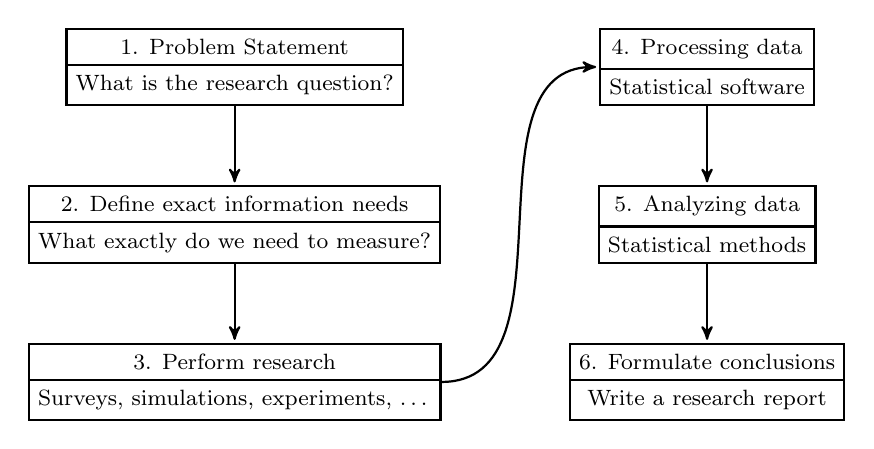
\begin{tikzpicture}[
      auto,
      thick,
      ->,
      >=stealth',
      shorten >=1pt,
      node distance=2cm,
      fase/.style={
        shape=rectangle split,
        rectangle split parts=2,
        ,
        draw}]
      
      
      \node[fase] (1) {
        \footnotesize{1. Problem Statement}
        \nodepart{second}
        \footnotesize{What is the research question?}
      };
      \uncover<2->{\node[fase] (2) [below of=1] {
          \footnotesize{2. Define exact information needs}
          \nodepart{second}
          \footnotesize{What exactly do we need to measure?}
        };}
      \uncover<3->{\node[fase] (3) [below of=2] {
          \footnotesize{3. Perform research}
          \nodepart{second}
          \footnotesize{Surveys, simulations, experiments, \ldots}
        };}
      \uncover<4->{\node[fase] (4) [right of=1, node distance=6cm] {
          \footnotesize{4. Processing data}
          \nodepart{second}
          \footnotesize{Statistical software}
        };}
      \uncover<5->{\node[fase] (5) [below of=4] {
          \footnotesize{5. Analyzing data}
          \nodepart{second}
          \footnotesize{Statistical methods}
        };}
      \uncover<6->{\node[fase] (6) [below of=5] {
          \footnotesize{6. Formulate conclusions}
          \nodepart{second}
          \footnotesize{Write a research report}
        };}
      
      \uncover<2->{\draw (1) -- (2);}
      \uncover<3->{\draw (2) -- (3);}
      \uncover<4->{\draw (3.east) to [out=0,in=180] (4.west);}
      \uncover<5->{\draw (4) -- (5);}
      \uncover<6->{\draw (5) -- (6);}
      \end{tikzpicture}
    \end{center}
  \end{columns}
  
\end{frame}

\section{Basic Concepts in Research}

\begin{frame}
  \frametitle{Variables and Values}
  
  \begin{description}
    \item[Variable] General property of an object, allows to distinguish objects
    \item[Value] Specific property, interpretation for that variable
  \end{description}
  
  \vspace{1cm}
  
  \begin{columns}[c]
    \column{.6\textwidth}
    \centering
    \includegraphics[width=.7\textwidth]{les1-07}
    
    \column{.4\textwidth}
    \fbox{\parbox{3cm}{%
        \scriptsize
        Variable: gender\\
        Value: male
    }}\\
    \vspace{.5cm}
    \fbox{\parbox{3cm}{%
        \scriptsize
        Variable: height\\
        Value: 180cm
    }}\\
    \vspace{.5cm}
    \fbox{\parbox{3cm}{%
        \scriptsize
        Variable: funny\\
        Value: no
    }}
    
  \end{columns}
\end{frame}

\begin{frame}
  \frametitle{Measurement Levels}
  
  \begin{itemize}
    \item = Variable types
    \item Determine most suitable method for analysis
    \begin{itemize}
      \item visualization methods
      \item central tendency and dispersion
      \item examine the relationship between variables
    \end{itemize}
  \end{itemize}
  
\end{frame}

\begin{frame}
  \frametitle{Measurement Levels}
  \framesubtitle{Qualitative vs quantitative}
  
  \begin{center}
    \begin{tabular}{ll}
    	\textbf{Qualitative}       & \textbf{Quantitative}        \\
    	\hline
        Not necessarily numeric    & Number + unit of measurement \\
    	Limited number of values   & Many values, often unique
    \end{tabular}
  \end{center}

  \bigskip

  Quantitative variables often contain the result of a \textbf{measurement}
\end{frame}

\begin{frame}
  \frametitle{Measurement Levels}
  \framesubtitle{Qualitative scales}
  
  \begin{description}
    \item[Nominal] Categories.
    
      e.g. gender, race, country, shape, \ldots
      
    \item[Ordinal] Order, rank.
    
      e.g. military rank, level of education, \ldots
  \end{description}
  
\end{frame}

\begin{frame}
  \frametitle{Measurement Levels}
  \framesubtitle{Quantitative scales}
  
  \begin{description}
    \item[Interval] No fixed zero point $\Rightarrow$ no proportions
    
    e.g. °C, °F
    
    \item[Ratio] Absolute zero point $\Rightarrow$ proportions
    
    e.g. distance (m), energy (J), weight (kg) \ldots\\
  \end{description}

  \bigskip

  Proportions:
  
  \begin{itemize}
    \item 20 m is 1/3th or $\sim$33\% longer than 15 m
    \item 20 °C is \textbf{NOT} 1/3th warmer than 15 °C (convert to °F)

  \end{itemize}    
  
\end{frame}

\begin{frame}
  \frametitle{Relations between variables}
  
  Variables are related if their values change \textbf{systematically}.
  
  \begin{center}
    \includegraphics[height=4cm]{les1-08a}
    \includegraphics[height=4cm]{les1-08b}
  \end{center}
\end{frame}

\begin{frame}
  \frametitle{Relations between variables: example}
  
  Is there a relationship between type of cola and taste appreciation?
  
  \begin{columns}
    \column{0.99\textwidth}
    \begin{table}
      \centering
      \begin{tabular}{l||c|c||c}
        & Pepsi & Coca Cola & Total \\
        \hline \hline
        Like & 56 & 24 & \alert<2>{80} \\
        \hline
        Dislike & 14 & 6 & \alert<2>{20} \\
        \hline \hline
        Total & \alert<2>{70} & \alert<2>{30} & \alert<2>{100}
      \end{tabular}
    \end{table}
    
    \only<2>{Marginal totals}
    
    \column{.01\textwidth}
    \hspace*{-2cm}
    \includegraphics[width=2cm]{les1-09}
  \end{columns}
\end{frame}

\begin{frame}
  \frametitle{Causal Relationships}
  
  Researchers are often looking for \textbf{causal relationships}, e.g.
  
  \begin{itemize}
    \item Frustration leads to agression
    \item Alcohol leads to decreased alertness
    \item \ldots
  \end{itemize}
  
  \begin{description}
    \item[Cause] Independent variable 
    \item[Consequence] Dependent variable
  \end{description}
\end{frame}

\begin{frame}
  \frametitle{Causal Relationships}
  \framesubtitle{Fake correlations or ``Spurious correlations''}
  
  \alertbox{\textcolor{yellow}{Warning!} A relationship between variables does not necessarily indicate a \emph{causal} relation!}
  
  \bigskip
  
  \begin{columns}
    \begin{column}{.8\textwidth}
      Examples:
      
      \begin{itemize}
        \item Violent video games lead to violent behaviour
        \item Vaccines can cause autism
        \item Relationship between drinking cola light and obesitas
        \item \ldots
      \end{itemize}
      
    \end{column}
    \begin{column}{.2\textwidth}
      \includegraphics[height=2.5cm]{les1-10}
    \end{column}
  \end{columns}

\end{frame}

\begin{frame}[plain]
  \centering
  \includegraphics[height=\textheight]{hst1-spurious-correlation}
\end{frame}

\section{Sample Testing}


\begin{frame}
  \large\bfseries
  
  USA Today has come out with a new survey. Apparently, three out of every four people make up 75\% of the population
  
  \bigskip
  
  ---David Letterman
  
\end{frame}

\begin{frame}
  \frametitle{Suppose you want to analyze a group of friends}
  
  Questions you can ask:
  
  \begin{itemize}
    \item How tall are my friends?
    \item What are their weights?
    \item How safe is their living environment?
    \item Do they have family?
    \item \ldots
  \end{itemize}

\end{frame}

\begin{frame}[plain]
  \frametitle{Population}
  
  \begin{figure}
    \centering
    \includegraphics[height=.9\textheight]{les5-heroes.jpg}
    \label{fig:les5-heroes}
  \end{figure}
  
\end{frame}


\begin{frame}[plain]
  \frametitle{Sample and Population}
  
  \begin{description}
    \item[Population] the collection of all objects/people/\ldots that you want to investigate 
    \item[Sample] a \textit{subset} of the population from which measurements will be taken
  \end{description}
  
  \begin{center}
    \begin{tikzpicture}[scale=.55]
    \fill[hgyellow] (2,2) ellipse (4cm and 2cm) ;
    \fill[hgorange] (1.5,2) ellipse (2cm and 1cm) ;
    \node[draw=none,minimum size=1cm,inner sep=0pt] at (3,0.5) {population};
    \node[draw=none,minimum size=1cm,inner sep=0pt] at (2.5,2) {sample};
    \end{tikzpicture}
  \end{center}

  \alertbox{Under certain circumstances, the results for a sample are representative for the population.}
\end{frame}

\begin{frame}
  \frametitle{Sample and Population}
  
  A sample is easier to analyze than the entire population
  
  \centering
  \begin{tikzpicture}[xscale=4,yscale=2]
  \draw (0,2) -- (0,0);
  \foreach \num/\label in {0/0, 0.2/20, .4/40, .6/60, .8/80, 1/100, 1.2/120, 1.4/140, 1.6/160, 1.8/180, 2/200}{%
    \draw (0, \num) -- (2.5, \num);
    \draw[shift={(0, \num)}] (1pt,0pt) -- (-1pt,0pt) node[left] {\scriptsize \label};
  }
  
  \node[anchor=north] (hero1) at (0.3,1.5)
  {\includegraphics[height=2.9cm]{les2-hero-1}};
  \node[anchor=north] (hero2) at (0.8,2.05)
  {\includegraphics[height=4cm]{les2-hero-2}};
  \node[anchor=north] (hero3) at (1.3,1.575)
  {\includegraphics[height=3.1cm]{les2-hero-3}};
  \node[anchor=north] (hero4) at (1.8,2.1)
  {\includegraphics[height=4.1cm]{les2-hero-4}};
  \node[anchor=north] (hero5) at (2.3,1.95)
  {\includegraphics[height=3.8cm]{les2-hero-5}};
  
  \node (size1) at (0.3, 1.5) {\scriptsize 141 cm};
  \node (size2) at (0.8, 2.1) {\scriptsize 198 cm};
  \node (size3) at (1.3, 1.51) {\scriptsize 143 cm};
  \node (size4) at (1.8, 2.15) {\scriptsize 201 cm};
  \node (size5) at (2.3, 1.95) {\scriptsize 184 cm};
  \end{tikzpicture}
\end{frame}


\begin{frame}
  \frametitle{Sampling Method}
  \begin{center}
    \begin{tikzpicture}[
    auto, thick, ->, >=stealth', shorten >=1pt, node distance=1.5cm,
    fase/.style={ shape=rectangle, fill=hgblue, text=white, draw}
    ]
    
    \node[fase] (1) { Definition of population };
    \node[fase] (2) [below of=1] { Define sampling frame };
    \node[fase] (3) [below of=2] { Choice of sampling method (budget and time) };
    
    \draw (1) -- (2);
    \draw (2) -- (3);
    \end{tikzpicture}
  \end{center}
  
\end{frame}

\begin{frame}
  \frametitle{Stratified to variables}
  
  \begin{center}
    \begin{tabular}{l|cccc|c}
      & \multicolumn{4}{c|}{\textbf{Age}} & \\
      Gender & $\le 18$ & $]18,25]$ & $]25, 40]$ & $> 40$ & Total\\
      \hline
      Woman & 500 & 1500 & 1000 & 250 & 3250 \\
      Man   & 400 & 1200 & 800 & 160 & 2560\\
      \hline
      Total & 900 & 2700 & 1800 & 410 & 5810
    \end{tabular}
    
    \vspace{.5cm}
    
    \pause
    \begin{tabular}{l|cccc|c}
      & \multicolumn{4}{c|}{\textbf{Age}} & \\
      Gender & $\le 18$ & $]18,25]$ & $]25, 40]$ & $> 40$ & Total\\
      \hline
      Woman & 50 & 150 & 100 & 25 & 325 \\
      Man   & 40 & 120 & 80 & 16 & 256\\
      \hline
      Total & 90 & 270 & 180 & 41 & 581
    \end{tabular}
    
  \end{center}
\end{frame}

\begin{frame}
  \frametitle{How to pick elements for a sample?}
  
  \begin{description}
    \item[Random sample]: every element from the population has an equal chance of being included in the sample.
    \item[Non-random sample]: the elements for the sample are \textit{not} randomly selected.
    Objects that can be collected \textit{easily} are more likely to be included (convenience sampling).
  \end{description}
  
  \begin{center}
    \includegraphics[height=.4\textheight]{les4-aselect}
  \end{center}
\end{frame}

\begin{frame}
  \frametitle{Possible Errors}
  
  Measurements in a sample will typically deviate from the value in the entire population $\Rightarrow$ Errors!
  
  \bigskip
  
  \begin{itemize}
    \item Accidentally $\leftrightarrow$ Systematic
    \item Sampling error $\leftrightarrow$ Non-sampling error
  \end{itemize}
\end{frame}

\begin{frame}
  \frametitle{Sampling Errors}
  
  \begin{itemize}
    \item<+-> Accidental sampling errors
    \begin{itemize}
      \item Pure coincidence
    \end{itemize}
    \item<+-> Systematic sampling errors
    \begin{itemize}
      \item Online survey: people without internet are excluded
      \item Street survey: only who is currently walking there
      \item Voluntary survey: only interested parties participate
    \end{itemize}
  \end{itemize}
\end{frame}

\begin{frame}
  \frametitle{Non-sampling Errors}
  \begin{itemize}
    \item<+-> Accidental non-sampling errors
    \begin{itemize}
      \item Incorrectly ticked answers
    \end{itemize}
    \item<+-> Systematic non-sampling errors
    \begin{itemize}
      \item Poor or non-calibrated measuring equipment
      \item Value can be influenced by the fact that you measure
      \item Respondents lie (number of cigarettes a day)
    \end{itemize}
  \end{itemize}
\end{frame}

\end{document}